\documentclass[../main.tex]{subfiles}

\title{Capitolo 2 - Teoria di Hodge}
\author{Edoardo Manini}
\date{Febbraio 20, 2025}

\begin{document}
\ifSubfilesClassLoaded{
\maketitle
\tableofcontents
}{}


In the first part of the thesis, we give an overview of Hodge thoery and Hodge structures stating basic results of the theory of variations of Hodge structures. We also give an introduction to mixed Hodge structures, which we use to study Hodge structures under degeneration.
Historically, Hodge structures were first developed to study compact Kähler manifolds, hence in this section we begin with a brief description of the Hodge decomposition, and then we give the definition of a (pure) Hodge structure.
\subsection{Hodge Decomposition}

Let $X$ be an $m$-dimensional compact oriented Riemannian manifold, denote the sheaf of smooth $n$-forms on $X$ by $\mathcal{A}^n_X$ and let $d\colon \mathcal{A}^n_X \to \mathcal{A}^{n+1}_X$ be the exterior derivative. Define the \emph{Laplacian}
\[\Delta_d = dd^\dag + d^\dag d,\]
where $d^\dag\colon \mathcal{A}^n_X \to \mathcal{A}^{n-1}_X$ is the \emph{codifferential}, the formal adjoint operator defined by $(d\alpha,\beta)=(\alpha,d^\dag\beta)$ or by $d^\dag = (-1)^{nm+m+1}*d*$, where $*$ denotes the Hodge star operator, the unique linear operator $*\colon \mathcal{A}^k_X \to \mathcal{A}^{m-k}_X$ with the property $\alpha\wedge*\beta=(\alpha,\beta)\eta$ where $\eta$ is the volume form.

Next define the set of \emph{harmonic forms of degree $n$} to be
\[\mathcal{H}^n(X) \defeq \{\alpha \in \mathcal{A}^n_X \mid \Delta_d\alpha = 0\}.\]
Then we have:

\begin{theorem}[Hodge's Theorem]  \textup{\cite[Thm. 5.23]{Voi07}} There is an isomorphism
\[\mathcal{H}^n(X) \cong H^n(X,\RR).\]
\end{theorem}


Now we turn to complex manifolds. Suppose $X$ is a complex manifold endowed with a Hermitian metric. We may decompose the sheaf of complex $n$-forms $\calA^n_X$ into a direct sum of sheaves of $(p,q)$-forms
\[
\calA^n_X = \bigoplus_{p+q=n} \calA^{p,q}_X
\]
and write $d = \partial + \bar {\partial}$, where $\partial\colon \calA^{p,q}_X \to \calA^{p+1,q}_X$ and $\bar {\partial}\colon \calA^{p,q}_X \to \calA^{p,q+1}_X$ are the \emph{Dolbeault operators}. In the same way as we defined the Laplacian, we may also define operators $\Delta_{\partial}$ and $\Delta_{\overline{\partial}}$, and these two operators both preserve the bidegree given by the decomposition of complex $n$-forms into $(p,q)$-forms. 
Nevertheless we note that, considering an arbitrary complex manifold with Hermitian metric, the two operators $\Delta_{\partial}$ and $\Delta_{\overline{\partial}}$ are not necessarily related to the Laplacian $\Delta_d$, and $\Delta_d$ does not necessarily preserve the bidegree. 

For this reason, we further restrict our attention to \emph{K\"{a}hler manifolds}. A Hermitian metric on a complex manifold $X$ is said to be \emph{K\"{a}hler} if its imaginary part $\omega$, which is a $(1,1)$-form on $X$, is closed. A complex manifold $X$ equipped with a K\"{a}hler metric is called a \emph{K\"{a}hler manifold} and the $2$-form $\omega$ on $X$ is the associated \emph{K\"{a}hler form}. 

The fact that K\"{a}hler manifolds provide the natural framework for Hodge theory relies on the observation that, on a K\"{a}hler manifold, the operator $\Delta_d$ preserves the bidegree. Indeed, if we define the \emph{Lefschetz operator} as $L\colon \calA^{p,q}_X \to \calA^{p+1,q+1}_X, \alpha \mapsto \alpha\wedge\omega$ with adjoint $L^\dag$, we have the following identities \cite[Prop. 6.5]{Voi07}: $[L^\dag,\partial]=i\Bar{\partial}^\dag$ and $[L^\dag,\Bar{\partial}]=-i\partial^\dag$ known as the \emph{Hodge identities} , from which we obtain:

\begin{theorem} \label{proportionality} If $X$ is a K\"{a}hler manifold, then 
\[\Delta_d = 2\Delta_{\partial}= 2\Delta_{\overline{\partial}}.\]
\end{theorem}
\begin{proof}
    We have
    \begin{align*}
    \Delta_d &= d d^\dag + d^\dag d = (\partial + \bar\partial)(\partial^\dag + \bar\partial^\dag) + (\partial^\dag + \bar\partial^\dag)(\partial + \bar\partial) \\
    &= \partial \partial^\dag +  \bar\partial \bar\partial^\dag + \partial^\dag \partial +  \bar\partial^\dag \bar\partial = \Delta_{\partial} + \Delta_{\bar \partial}
    \end{align*}
    because $\partial \bar\partial^\dag + \bar\partial^\dag \partial =0$ since, using the Hodge identities, we have
    \[
    i (\partial \bar\partial^\dag + \bar\partial^\dag \partial) = \partial (L^\dag \partial -  \partial L^\dag) + (L^\dag \partial -  \partial L^\dag) \partial \stackrel{\partial^2 = 0}{=} 0
    \]
    It remains to show that $\Delta_{d} = 2 \Delta_{\partial}$:
    \begin{align*}
    \Delta_{d} &=  (\partial + \bar\partial)(\partial^\dag + \bar\partial^\dag) + (\partial^\dag + \bar\partial^\dag)(\partial + \bar\partial) \\
    &=  (\partial + \bar\partial)(\partial^\dag - i [L^\dag , \partial]) + (\partial^\dag - i [L^\dag , \partial] )(\partial + \bar\partial) \\
    &= \partial \partial^\dag +  \bar\partial \partial^\dag + i  \bar\partial \partial L^\dag -i \bar\partial  L^\dag \partial +  \partial^\dag \partial + \partial^\dag \bar\partial - i   L^\dag  \partial \bar\partial + i \partial   L^\dag  \bar\partial
    \end{align*}
    and since $\partial^\dag = i [L^\dag,\Bar{\partial}]$, we obtain 
    \[
    \partial^\dag \bar\partial = -i \bar\partial  L^\dag \bar\partial = -\bar\partial \partial^\dag.
    \]
    Thus
    \[
    \Delta_{d} = \Delta_{\partial} + i \partial [L^\dag , \bar\partial] + i  [L^\dag , \bar\partial] \partial = 2 \Delta_{\partial}.
    \]
\end{proof}


This imply the following.

\begin{cor}  \textup{\cite[Cor. 6.9]{Voi07}} If $\alpha$ is a harmonic form of degree $n$ on a K\"{a}hler manifold $X$, then the components of $\alpha$ of type $(p,q)$ are also harmonic.
\end{cor}

Hence, we have a decomposition
\[\calH^k(X) = \bigoplus_{p+q=k}\calH^{p,q}(X),\]
where $\calH^{p,q}(X)$ denotes the space of harmonic forms of type $(p,q)$, and this decomposition satisfies $\calH^{p,q}(X) = \overline{\calH^{q,p}(X)}$ \cite[Cor. 6.10]{Voi07}.

Ultimately, assuming also that $X$ is compact, we then have $\calH^k(X) \cong H^k(X,\CC)$ and the previous decomposition induces a decomposition 
\[
H^k(X,\CC) = \bigoplus_{p+q=k}H^{p,q}(X).
\]
The spaces in this decomposition are related to the cohomology of the sheaves of holomorphic forms  $\Omega^p_X$.
\begin{theorem} [Dolbeault's isomorphism] \label{DolbIso} \textup{\cite[Lemma 6.18]{Voi07}}
\[
H^{p,q}(X) \simeq H^q(X,\Omega^p_X).
\]
\end{theorem}
\begin{proof}
Let $\calA^{p,q}_X$ denote the sheaf of differential $(p, q)$-forms on $X$. The $q$-th cohomology group $H^q(X,\Omega^p)$ can be calculated via the acyclic resolution:
\[
0 \lra \Omega^p_X \xrightarrow{\bar \partial}  \calA^{p,0}_X \xrightarrow{\bar \partial}  \calA^{p,1}_X \xrightarrow{\bar \partial}  \calA^{p,2}_X \xrightarrow{\bar \partial} \cdots
\]
which is acyclic because the sheaves $\calA^{p,q}$ are soft since they are $\calC^\infty$-modules and $\calC^\infty$ is soft and is exact since locally a $\bar \partial$-Poincarè Lemma holds.
Then 
\[
H^q(X,\Omega^p_X) \simeq H^q \left( \calA^{p,q-1}(X) \xrightarrow{\bar \partial}  \calA^{p,q}(X) \xrightarrow{\bar \partial}  \calA^{p,q+1}(X) \right)
\]
which is the group of  $\bar \partial$-closed $(p, q)$ forms modulo exact forms. This is isomorphic to the space of $\Delta_{\bar \partial}$-harmonic $(p, q)$-forms.
By Thm. \ref{proportionality}, this is the same as the space of harmonic (p, q)-forms $H^{p,q}(X)$.
\end{proof}

We obtain:

\begin{theorem}[Hodge Decomposition] \label{hodgedecomp} Let $X$ be a compact K\"{a}hler manifold. We have
\begin{align}
        H^k(X,\CC) &= \bigoplus_{p+q=k} H^{p,q}(X) \label{eq:eq1}\tag{Hodge Decomposition} \\
        H^{p,q}(X) &= \overline{H^{q,p}(X)} \label{eq:eq2}\tag{Hodge Symmetry}
\end{align}
where $H^{p,q}(X) \cong H^q(X,\Omega^p_X)$.
\end{theorem}


This Hodge Decomposition Theorem sets limitations on the cohomology of a K\"{a}hler manifold, as displayed by the next

\begin{cor}
For every compact K\"{a}hler manifold $X$, the odd Betti numbers $b_{2k-1}(X)$ are even.
\end{cor}

The Hodge numbers $h^{p,q}(X) \defeq \dim_\CC H^{p,q}(X)$ of a compact K\"{a}hler manifold $X$ are usually arranged in the \emph{Hodge diamond}:
\begin{center}
\begin{tikzpicture}[scale=1]
\draw (4,0) node              {$h^{0,m}(X)$};
\draw (-4,0) node             {$h^{m,0}(X)$};
\draw (2,0) node              {$h^{1,m-1}(X)$};
\draw (-2,0) node             {$h^{m-1,1}(X)$};
\draw (0,0) node              {$\cdots$};
\draw (3,1) node              {$\ddots$};
\draw (0,1) node              {$\vdots$};
\draw (-3,1) node             {$\iddots$};
\draw (3,-1) node             {$\iddots$};
\draw (0,-1) node             {$\vdots$};
\draw (-3,-1) node            {$\ddots$};
\draw (4/3,2) node            {$h^{m-1,m}(X)$};
\draw (-4/3,2) node           {$h^{m,m-1}(X)$};
\draw (4/3,-2) node           {$h^{0,1}(X)$};
\draw (-4/3,-2) node          {$h^{1,0}(X)$};
\draw (0,3) node              {$h^{m,m}(X)$};
\draw (0,-3) node             {$h^{0,0}(X)$};
\draw (16/3,0) -- (0,4) -- (-16/3,0) -- (0, -4) -- cycle;
\end{tikzpicture}
    \label{HODGE_diamond}
\end{center}
    
where $m = \dim_{\CC}(X)$.
Hodge symmetry tells us that this diamond is symmetric along its vertical axis $h^{p,q}(X) = h^{q,p}(X)$; while Hodge decomposition tells us the $k$-th Betti number $b_k(X) = \sum_{p+q=k}h^{p,q}(X)$ is the sum of the numbers on the horizontal line $p+q=k$. By Poincaré duality, there is a perfect pairing $H^k(X,\CC) \otimes H^{2m-k}(X,\CC) \to \CC$ sending $\alpha \otimes \beta$ to $\int_X \alpha\wedge \beta$. Let $\alpha = \alpha_{pq} \in \calH^{p,q}(X) \subseteq \calA^i_X$ and $\beta = \sum_{p^\prime+q^\prime=i} \beta_{m-p^\prime,m-q^\prime} \in \calH^{2m-i} (X) \subseteq \calA^{2m-i}_X$. Then $\alpha \wedge \beta =\alpha \wedge \beta_{m-p,m-q} $, i.e. Poincaré duality preserves the bidegree. Hence $H^{m-p,m-q}(X) \cong H^{p,q}(X)^*$, so $h^{p,q}(X) = h^{m-p,m-q}(X)$. That means that the Hodge diamond is symmetric under rotation of 180°, and combining the two symmetries results in symmetry along the horizontal axis.

\begin{es} For a curve $C$ of genus $g$, it is not hard to see that its Hodge diamond is given by
\[
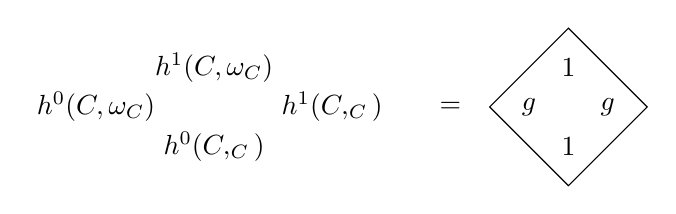
\begin{tikzpicture}[scale=1]
\draw (-1.5,0) node          {$h^1(C,\calO_C)$};
\draw (-4.5,0) node         {$h^0(C,\omega_C)$};
\draw (-3,0.5) node          {$h^1(C,\omega_C)$};
\draw (-3,-0.5) node         {$ h^0(C,\calO_C)$};
\draw (0,0) node         {$=$};
\draw (2,0) node              {$g$};
\draw (1,0) node             {$g$};
\draw (1.5,0.5) node              {$1$};
\draw (1.5,-0.5) node             {$1$};
\draw (2.5,0) -- (1.5,1) -- (0.5,0) -- (1.5, -1) -- cycle;
\end{tikzpicture}
\]
where we denote with $\omega_C$ the \emph{canonical bundle} $\Omega^{\dim(C)}_C$ of $C$.
\end{es}

For a generic \emph{Calabi-Yau} manifold, i.e. a smooth compact  K\"{a}hler manifold with trivial canonical bundle, Serre duality  \cite[Thm. 5.32]{Voi07}, $H^q(X,\calE) \cong H^{m-q}(X,\calE^* \otimes \omega_X )^*$ for a holomorphic vector bundle $\calE$, implies that $h^{0,i}(X)=h^i(X,\calO_X)=h^{m-i}(X,\calO_X^* \otimes\omega_X) =h^{m-i}(X,\calO_X)= h^{0,m-i}(X)  $, which says that the edges of the diamond are each symmetric.
$1$-dimensional Calabi-Yau manifolds are elliptic curves, i.e. curves of genus $1$. An interesting class of $2$-dimensional Calabi-Yau manifolds are $K3$ surfaces.

\begin{es} \label{K3Hodgeex} Suppose $S$ is a K3 surface, meaning a smooth compact complex surface with trivial canonical bundle and vanishing $H^1(S,\calO_S) = 0$ (or equivalently vanishing first Betti number $b_1(S)=0$). Using the symmetries along the edges and the fact that $\chi_{top}(X)=24$, the Hodge diamond of $S$ results 
\[
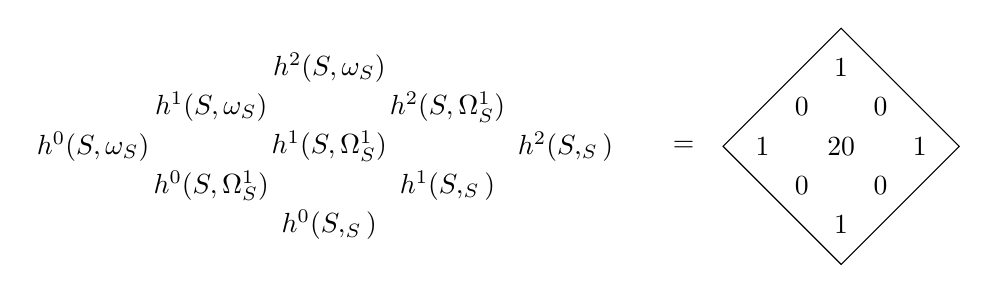
\begin{tikzpicture}[scale=1]
\draw (-5,0) node         {$h^0(S,\omega_S)$};
\draw (-2,0) node          {$h^1(S,\Omega^1_S)$};
\draw (1,0) node         {$h^2(S,\calO_S)$};
\draw (-3.5,0.5) node          {$h^1(S,\omega_S)$};
\draw (-0.5,0.5) node          {$h^2(S,\Omega^1_S)$};
\draw (-3.5,-0.5) node         {$ h^0(S,\Omega^1_S)$};
\draw (-0.5,-0.5) node         {$ h^1(S,\calO_S)$};
\draw (-2,1) node          {$h^2(S,\omega_S)$};
\draw (-2,-1) node         {$h^0(S,\calO_S)$};
\draw (2.5,0) node         {$=$};
\draw (3.5,0) node               {$1$};
\draw (4.5,0) node               {$20$};
\draw (5.5,0) node               {$1$};
\draw (4,0.5) node              {$0$};
\draw (5,0.5) node              {$0$};
\draw (4,-0.5) node             {$0$};
\draw (5,-0.5) node             {$0$};
\draw (4.5,1) node               {$1$};
\draw (4.5,-1) node              {$1$};
\draw (6,0) -- (4.5,1.5) -- (3,0) -- (4.5, -1.5) -- cycle;
\end{tikzpicture}
\]


\end{es}

\begin{es} \label{CY3Hodgeex} Let now $X \subseteq \CC\Proj^4$ be a quintic threefold. It is Calabi-Yau since, by the adjunction formula, $\omega_X=\calO_X(-5+5)=\calO_X$ and by Lefschetz hyperplane Theorem $h^i (X, \calO_X) = 0$ for $0 < i < 3$ as well as $h^{1,1}(X) =1$ . From the symmetry along the edges coming from Serre duality and the fact that  $\chi_{top}(X)=-200$, we obtain the following Hodge diamond:
\[\begin{array}{ccccccc}
& & & 1 & & & \\
& & 0 &  & 0 & & \\
& 0\  & & 1 & &\  0 & \\
1\quad &  & 101 & & 101 & &\quad 1\\
& 0\  & & 1 & &\ 0 & \\
& & 0 & & 0 & & \\
& & & 1 & & &
 \end{array}
\]

We will see that a consequence of the mirror symmetry conjecture is that, for a mirror pair of Calabi-Yau threefolds $X$ and $\check{X}$, the two Hodge numbers in the center are interchanged:
\[h^{2,1}(X) = h^{1,1}(\check{X}),  \qquad h^{1,1}(X) = h^{2,1}(\check{X}).\]
\end{es}

\begin{es}
Note that the K\"{u}nneth formula is compatible with the Hodge decomposition, i.e. 
\[
H^{p,q}(X \times Y ) \simeq \bigoplus_{p_1+p_2=p \atop q_1+q_2=q} H^{p_1,q_1}(X) \otimes H^{p_2,q_2}(Y).
    \]
Hence we can calculate the Hodge diamond of a product of a genus $g$ curve $T^g$ with a genus $g^\prime$ curve $T^{g^\prime}$. Using the formula for Hodge numbers 
\[
h^{p,q}(X \times Y ) = \sum_{p_1+p_2=p \atop q_1+q_2=q} h^{p_1,q_1}(X) \cdot h^{p_2,q_2}(Y)
\]
we find the Hodge diamond for $T^g \times T^{g^\prime} $:
\[
\begin{array}{ccccc} & & 1 & & \\
& g + g^\prime & & g + g^\prime &  \\
g g^\prime & & 2g g^\prime + 2  & & g g^\prime \\
&  g + g^\prime & &  g + g^\prime & \\
& & 1 & &  
\end{array}\]


\end{es}


\subsection{Lefschetz Decomposition}

Now we embark on a short detour to present another major decomposition of the cohomology of a compact K\"{a}hler manifold: the \emph{Lefschetz decomposition}. Let $X$ be a compact K\"{a}hler manifold, then since the \emph{Lefschetz operator}, i.e. wedging with the K\"{a}hler form, commutes with the differential we get an induced map in cohomology
\[L \colon H^n(X,\CC) \longrightarrow H^{n+2}(X,\CC).\]
We have:

\begin{theorem}[Hard Lefschetz] \textup{\cite[Sect. 6.2.3]{Voi07}} 
\label{HardLef}
Let $X$ be a compact K\"{a}hler manifold of dimension $m$. Then
\begin{align} \label{Lef}
    L^{m-n}\colon H^n(X,\CC) \longrightarrow H^{2m-n}(X,\CC)
\end{align}
\[ \left( \text{ or } L^{k}\colon H^{m-k}(X,\CC) \longrightarrow H^{m+k}(X,\CC) \right)\]

is an isomorphism. Furthermore, if $n \leq j \leq m$, then
\[
L^{m-j}\colon H^n(X,\CC) \longrightarrow H^{2m+n-2j}(X,\CC)
\]
\[ \left( \text{ or } 
L^{s}\colon H^{m-k}(X,\CC) \longrightarrow H^{m-k+2s}(X,\CC) \quad \text{ for } \quad 0 \leq s \leq k \right)
\]
is injective.
\end{theorem}
In the Hodge diamond, $L$ corresponds to moving up $1$ step along the vertical lines. The isomorphism \eqref{Lef} takes the $(p,q)$-slot to its reflection about the horizontal central line. Thus, the Hodge diamond of a compact K\"{a}hler manifold is symmetric about the horizontal diagonal, a phenomenon which we have already observed.

The Hard Lefschetz Theorem dispense more restrictions on the topology of complex manifolds that admit a K\"{a}hler structure:

\begin{cor} If $m = \dim X$, the odd Betti numbers $b_{2k-1}(X)$ increase with $k$ for $2k - 1 \leq m$ and, similarly, the even Betti numbers $b_{2k}(X)$ increase for $2k \leq m$.
\end{cor}

By the Hard Lefschetz Theorem, $k+1$ is the smallest value of $s$ such that the homomorphism
\[
 L^s \colon H^{m-k}(X) \to H^{m-k+2s}(X)
\]
may have a kernel.
For each $k=0,1,\dots,m$, set $n=m-k$ and define
\[
P^{m-k}(X,\CC) \defeq \ker(L^{k+1}\colon H^{m-k}(X,\CC) \longrightarrow H^{m+k+2}(X,\CC))
\]
to be the \emph{$n$-th primitive cohomology of $X$}. By the Hard Lefschetz Theorem,
\[
 H^{m-k}(X,\CC) = P^{m-k}(X) \oplus L \left( H^{m-k-2}(X,\CC) \right).
\]
Thus we have:

\begin{theorem}[Lefschetz Decomposition] \textup{\cite[Cor. 6.26]{Voi07}} 
\label{LefDec}
Let $X$ be a compact K\"{a}hler manifold of dimension $m$. Then for any $n$ there is a decomposition
\[H^n(X,\CC) = \bigoplus_{s \geq 0 \atop 0 \leq n-2s \leq m} L^sP^{n-2s}(X,\CC).\]
\end{theorem}

\subsection{Hodge Structures}    

Hodge structures basically compress multiple invariants and comparison isomorphisms between them in one single item.
They are useful for different reasons. They are finer invariants than for instance singular cohomology: Hodge structures can differentiate two non-isomorphic elliptic curves while singular cohomology cannot since they are homeomorphic.

Here is the definition of a (pure) Hodge structure:

\begin{defn} A (\emph{pure}) \emph{Hodge structure of weight $n \in \Z$}, denoted $(H_{\Z},H^{p,q})$, consists of a finitely generated free abelian group $H_{\Z}$ (a \emph{lattice}) along with a decomposition $H_{\CC} = \bigoplus_{p+q = n} H^{p,q}$ of the complexification  $H_\CC := H_{\Z} \otimes_{\Z} \CC$, which satisfies $H^{p,q} = \overline{H^{q,p}}$.
\end{defn}

We could also introduce the notion of rational (resp. real) Hodge structures, obtained by replacing the lattice $H_{\Z}$ with a rational (resp. real) vector space. Furthermore, one could generalize this notion to allow Hodge structures on $R$-modules $H_R$ of finite type, with $R \subset \mathbb{R}$ a noetherian subalgebra. 

\begin{es}
Let $H_{\CC} = H^{k,k}$ and $H^{p,q} = 0, (p, q) \neq (k, k)$. One then gets the simplest example of a Hodge structure, called a \emph{trivial Hodge structure of weight $2k$}.
\end{es}

\begin{es} We get a new Hodge structure if we let $H_{\Z} = 2\pi i \Z$ (considered as a subgroup of $\CC$) and $H_{\CC} = H^{-1,-1}$. This is a pure Hodge structure of weight $-2$ and is actually the unique $1$-dimensional pure Hodge structure of weight $-2$ up to isomorphism. It is called the \emph{Tate Hodge structure} and is often denoted by $\Z (1)$.
\end{es}


\begin{es}
From the Hodge decomposition theorem \ref{hodgedecomp} for $X$ a compact K\"{a}hler manifold, we see that letting $H_{\ZZ}(X):=H^n(X,\Z)/\mathrm{torsion}$, then the data $(H_{\Z}(X),H^{p,q}(X))$ defines a pure Hodge structure of weight $n$. 
\end{es}


It is also common to see a pure Hodge structure of weight $n$ defined by a decreasing filtration, called the \emph{Hodge filtration}, $\{F^p\}$ on $H_\CC$
\[ H_\CC = F^0 \supset F^1 \supset \cdots \supset F^n \supset \{0\}\]
that satisfies $ H^{p,q} = {F^p} \cap \overline{F^q} $ and $H_\CC \simeq F^p \oplus \overline{F^{n-p+1}}$. The two definitions are completely equivalent: given a decomposition $H_\CC = \bigoplus_{p+q = n} H^{p,q}$ we may define a filtration by setting $F^p := H^{n,0} \oplus \cdots \oplus H^{p,n-p}$. We see that for every $i$, $\overline{F^i} =  \bigoplus_{j \geq i} H^{n-j,j} $, hence letting $q = n-p$, we have  ${F^p} \cap \overline{F^q} = ( H^{n,0} \oplus \cdots \oplus H^{p,q} ) \cap (H^{p,q} \oplus \cdots \oplus H^{0,n} )
= H^{p,q}$ and  ${F^p} \cap \overline{F^{q+1}} = ( H^{n,0} \oplus \cdots \oplus H^{p,q} ) \cap (H^{p-1,q+1} \oplus \cdots \oplus H^{0,n} ) = 0$, so ${F^q} + \overline{F^{q+1}} = {F^q} \oplus \overline{F^{q+1}} = \bigoplus_{p=0}^n H^{p,q} = H_\CC $ as desired.
Given a filtration $\{F^p\}$ satisfying $ F^p \oplus \overline{F^{n-p+1}} \simeq H_\CC $ , we may define a decomposition by setting $H^{p,q} := F^p \cap \overline{F^q}$. Note that in this case we see $\overline{H^{q,p}} = \overline{ F^q \cap \overline{F^p} } = \overline{ F^q} \cap {F^p}  = H^{p,q} $ which is the property satisfied by a Hodge structure.

The Hodge filtration will prove to be a useful reformulation when we come to study Hodge structures associated to compact K\"{a}hler varieties, as it varies holomorphically in families. 
The polynomial
\begin{align}
e_{Hdg}(H) = \sum_{p,q \in \Z} h^{p,q}(H)u^pv^q \label{HdgPol}
\end{align}
is the associated \emph{Hodge number polynomial}.


Given Hodge structures $V,W$ of weight $n$ and $m=n+2r$, a morphism of Hodge structures of bidegree (or type) $(r,r)$ is a morphism $f \colon V \to W$ of $\Z$-modules whose complexification maps $V^{p,q}$ to $W^{p+r,q+r}$. A morphism of Hodge structures of bidegree $(0,0)$ is simply called a morphism of Hodge structures.

\begin{es}
    Let $X$ and $Y$ be two compact K\"{a}hler manifolds and let $f \colon X \to Y$ be a holomorphic map. Then $f^* \colon  H^n(Y,\Z) \to H^n(X, \Z)$ is a morphism of Hodge
structures of bidegree $(0, 0)$.

The Gysin morphism $f_! \colon H^n(X, \Z) \to H^{n-2r}(Y,\Z)$ is also a morphism of Hodge structures of bidegree $(r, r)$, where $r = \dim_\CC(Y) - \dim_\CC(X)$.
\end{es}

To produce different Hodge structures starting from given ones, it is natural to use the following multi-linear algebra constructions:
\begin{enumerate}
\item Let $(H_{\Z},H^{p,q})$, $(H'_{\Z},H'^{p,q})$ be two Hodge structures, both of weight $n$. Then we can define their direct sum by taking the underlying lattice to be the direct sum of the two lattices $H_{\Z} \oplus H'_{\Z}$, and the $(p, q)$-components to be the direct sums of the $(p, q)$-components of each term $H^{p,q} \oplus H'^{p,q}$. The direct sum is thus a Hodge structure of weight $n$.
\item The dual of a Hodge structure $(H_{\Z},H^{p,q})$ of weight $n$ is a Hodge structure of weight $-n$, defined by taking as underlying lattice the dual $H_\Z^\vee := \Hom (H_\Z, \Z)$ with the dual Hodge decomposition $(H^{\vee})^{p,q} = (H^{-p,-q})^\vee.$ 
\item Let $(H_{\Z},H^{p,q})$, $(H'_{\Z},H'^{p,q})$ be two Hodge structures of weight $n$ and $n'$ respectively. Then we can define their tensor product by taking as underlying lattice $H''_{\Z} = H_{\Z} \otimes H'_{\Z}$ and defining the Hodge decomposition on its complexification as:
\[
H''^{p,q} = \bigoplus_{\substack{r+r' = p\\ s+s'=q}} H^{r,s} \otimes H'^{r',s'}. 
\]
The tensor product is a Hodge structure of weight $n + n'$ with Hodge number polynomial given by
\begin{align}
    e_{Hdg}(H \otimes H^\prime) = e_{Hdg}(H)e_{Hdg}(H^\prime). \label{ProdHdgPol} 
\end{align}
\item From the previous two constructions it immediately follows that, for Hodge structures $(H_{\Z},H^{p,q})$ and $(H'_{\Z},H'^{p,q})$ of weights $n$ and $n'$, we also have Hodge structures on $\Hom(H_\Z , H'_\Z ) = H_\Z^\vee \otimes H'_\Z$  of weight $n'-n$ and on $\mathrm{Sym}^k (H_\Z )$ and $\bigwedge^k H_\Z$, both of weight $kn$.
\end{enumerate}

\begin{es} \label{TateTwistDef}
Starting from a Hodge structure $(H_{\Z}, H^{p,q})$ of weight $n$, we can produce a new Hodge structure of weight $n - 2r$, which is referred to as the \emph{$r$-th Tate twist} of the original Hodge structure, by setting
\[
H(r)_{\Z} = H_{\Z}, \quad H(r)^{p,q} = H^{p+r,q+r}. 
\]
In terms of the Hodge filtration, we have
\[
F^p H(r)_\CC = F^{p+r} H_\CC.
\]
\end{es}

Morphisms of Hodge structures preserve the Hodge filtration since for $V,W$ Hodge structures of the same weight $n$, $f_\CC(F^p V) = f_\CC(\bigoplus_{i \geq p} V^{i,n-i})= \bigoplus_{i \geq p} f_\CC(V^{i,n-i}) \subseteq \bigoplus_{i \geq p} W^{i,n-i} =F^p W  $. The converse is also true:
\begin{proposition} \label{morHS}
     Let $V,W$ be Hodge structures of weight $k$. Suppose that
$f \colon V \to W$ is a linear map preserving the $\Z$-structures and such that
\[
f_\CC(F^pV ) \subseteq F^pW.
\]
Then $f$ is a morphism of Hodge structures.
\end{proposition} 
\begin{proof}
    One has $f_\C (\overline{F^q V}) \subseteq \overline{F^q W}$, so, if $p + q = k$, we have
    \[
f_\C(V^{p,q}) = f_\C(F^pV \cap \overline{F^qV} ) \subseteq F^pW \cap \overline{F^qW} = W^{p,q}. 
    \]
\end{proof}

The above proposition shows that the category of pure Hodge structures of weight $n$ is equivalent to the
category of finitely generated abelian groups whose complexifications have finite decreasing Hodge filtrations, (i.e. satisfying $H_\CC \simeq F^p \oplus \overline{F^{n-p+1}}$), with morphisms being homomorphisms $f$ of abelian groups whose
complexifications $f_\CC$ preserve the filtrations.

Thanks to the Hodge direct sum decomposition, we have that a morphism of Hodge structure is strict with respect to the Hodge filtration, namely $f(F^pV) = \im(f) \cap F^pW$.

This means that for an injective morphism of Hodge structures $f \colon V \hra W$, the induced morphism on the graded pieces $f \colon \Gr^p_F V \hra \Gr^p_F W$ is also injective.

Clearly, the image of a morphism of Hodge structures is again a Hodge structure. By the above constructions, the duality operation preserves Hodge structures, and one can show that the kernel of a morphism of Hodge structures is a Hodge structure:

 \begin{lemma}
     Let $f \colon V \to W $ be a morphism of Hodge structures of type $(r,r)$ and let $K_\Z := \ker f \subset V_\Z, K_\CC := \ker f_\CC $. Setting $F^pK_\CC \defeq K_\CC \cap F^pV_\CC$, then $(K_\Z, F^p K_\CC)$ is a Hodge structure.
 \end{lemma}
 \begin{proof}
     We show that if $K^{p,q} \defeq F^pK_\CC \cap \overline{F^q K_\CC}$ where $p+q=n$, we obtain $K_\CC = \bigoplus_{p+q=n} K^{p,q}$. If $\alpha \in K_\CC \subset V_\CC = \bigoplus_{p+q=n} V^{p,q}$, then $\alpha$ has a Hodge decomposition in $V_\CC$ as $\alpha = \sum_{p+q=n} \alpha^{p,q}$. Then $f(\alpha)=0=\sum_{p+q=n}f(\alpha^{p,q})$, with  $f(\alpha^{p,q}) \in W^{p+r,q+r}$. Thus, $f(\alpha^{p,q})=0$ so $\alpha^{p,q} \in K^{p,q}$.
 \end{proof}

 
 Using the preceding multi-linear algebra constructions, it is not hard to see that we in fact have:
\begin{cor}
    The category of Hodge structures is an abelian category
which we denote $\mathfrak{hs}$.
\end{cor}
Recall the construction of the Grothendieck group $K_0$. 
It is defined for any abelian category such as the category $\mathfrak{hs}$ of Hodge structures: it is the free group on the isomorphism classes $[H]$ of Hodge structures $H$ modulo
the subgroup generated by $[H] - [H^\prime] - [H^{\prime\prime}]$ where $0 \to H^\prime \to H \to H^{\prime\prime} \to 0$ is a short exact sequence of Hodge structures. It carries a ring structure coming from the tensor product. Because the Hodge number polynomial (\ref{HdgPol}) is
clearly additive and by (\ref{ProdHdgPol}) behaves well on products, we have: 
\begin{lemma}
    The Hodge number polynomial defines a ring homomorphism
    \[
    e_{Hdg} \colon K_0(\mathfrak{hs}) \to Z[u, v, u^{-1},v^{-1}].
    \]
Inside $K_0(\mathfrak{hs})$, Tate twisting $r$-times can be expressed as $[H] \mapsto [H] \cdot  \LL^{-r}$ where
\begin{align}
    \LL = H^2(\PP^1) \in K_0(\mathfrak{hs}). \label{L}
\end{align}
\end{lemma} 



\subsection{Fr\"{o}licher Spectral Sequence}
Now we use the theory of spectral sequences and hypercohomology, which we recall in the appendix \ref{SpSeq}, to give a weaker form of the Hodge decomposition theorem valid for all complex manifolds.
Let $X$ be a complex manifold (not necessarily K\"{a}hler), consider the holomorphic de Rham complex $(\Omega^\bullet_X, \partial)$. Provide it with the stupid (trivial, b\^{e}te) filtration given by
\[
\sigma^p \Omega^\bullet_X = \Omega^{\geq p}_X = 0 \longrightarrow \cdots \longrightarrow 0 \longrightarrow \Omega^p_X \stackrel{\partial}{\longrightarrow} \Omega^{p+1}_X \stackrel{\partial}{\longrightarrow} \cdots. 
\]
To define our spectral sequence, note first that the double complex $(\calA^{p,q}_X,\partial,(-1)^p \bar {\partial})$ provides an acyclic resolution of $\Omega^{\bullet}_X$
\begin{center}
\centerline{
\xymatrix
{
 & \vdots&\vdots&\vdots\\
0 \ar[r] & \calA_X^{0,1} \ar_{\partial}[r]\ar_{\overline{\partial}}[u]& \calA_X^{1,1} \ar_{\partial}[r]\ar_{-\overline{\partial}}[u]& \calA_X^{2,1} \ar_{\partial}[r]\ar_{\overline{\partial}}[u]&\cdots\\
0 \ar[r] & \calA_X^{0,0} \ar_{\partial}[r]\ar_{\overline{\partial}}[u]& \calA_X^{1,0} \ar_{\partial}[r]\ar_{-\overline{\partial}}[u]& \calA_X^{2,0} \ar_{\partial}[r]\ar_{\overline{\partial}}[u]&\cdots\\
0 \ar[r] &  
\Omega_X^0 \ar_{\partial}[r]\ar[u]& 
\Omega_X^1 \ar_{\partial}[r]\ar[u]&
\Omega_X^2 \ar_{\partial}[r]\ar[u]&\cdots\\
 & 0 \ar[u] & 0 \ar[u] & 0 \ar[u]
}}
\end{center}
and the associated total complex is exactly the de Rham complex $\calA_X^{\bullet}$ with the exterior derivative $d = \partial + \overline{\partial}$.

The filtration $\sigma^p\Omega^\bullet_X$ lifts to a filtration on the double complex $\calA_X^{\bullet,\bullet}$, which in turn gives a filtration $\sigma^p\calA^{\bullet}_X$ on the de Rham complex $(\calA^{\bullet}_X,d)$ by
\[\sigma^p\calA^n_X := \bigoplus_{\substack{i \geq p \\ i+j = n}} \calA^{i,j}_X = \bigoplus_{\substack{i = p}}^n \calA^{i,n-i}_X.\]

We get an induced filtration on the hypercohomology of $(\Omega_X^{\bullet},\partial)$, as described in \ref{HypCoh}. We denote the filtration by $F^p\mathbb{H}^n (X, \Omega^\bullet_X)$.  Furthermore, since the de Rham complex is an acyclic resolution of the locally constant sheaf $\CC_X$, \cite[Cor. 8.14]{Voi07}, we have that the hypercohomology of this complex of sheaves calculates the cohomology of $X$, i.e. $\mathbb{H}^n(X,\Omega_X^{\bullet}) = H^n(X,\CC)$ . By this, we define an equivalent of the Hodge filtration on the cohomology of $X$ using the filtration on the hypercohomology
\[F^p H^n(X, \CC) \defeq F^p\mathbb{H}^n (X, \Omega^\bullet_X).\]

Moreover, by Thm. \ref{thm:specseq}, to the filtered complex $(\calA_X^{\bullet},\sigma)$ we can associate a spectral sequence
\begin{align*}
E_0^{p,q} = \Gamma(X,\calA_X^{p,q}) &\Rightarrow  \HH^{p+q}(X,\Omega_X^{\bullet}) \\
\text{ i.e. } E_\infty^{p,q} &= \Gr_F^p \HH^{p+q}(X,\Omega_X^{\bullet}) = \frac{F^pH^{p+q}(X,\CC)}{F^{p+1}H^{p+q}(X,\CC)}.
\end{align*}
This sequence is called the 
\emph{Fr\"{o}licher spectral sequence}.
It is a rightward oriented (see rem. \ref{spseqorientation}) spectral sequence. the differential $d_0$ is just the morphism in the vertical direction $\bar \partial$ and in the first page $d_1$ is nothing but $\partial$, the horizontal morphism.

Impose now the assumption that the Fr\"{o}licher spectral sequence degenerates at $E_1$. We have that $E_1^{p,q} = H^{p,q}_{\bar\partial}(X) \simeq H^q(X,\Omega_X^p)$, where we used Dolbeault's isomorphism \ref{DolbIso}. By $E_\infty = E_1$, we deduce
\[
H^q(X,\Omega_X^p) = F^pH^{p+q}(X,\CC)\, / \, F^{p+1}H^{p+q}(X,\CC).
\]
Because a short exact sequence of vector spaces is always split, we can write $H^n(X,\CC)$ as a direct sum of graded pieces of any finite filtration. Indeed, we obtain a decomposition
\[
H^n(X,\CC) \simeq \bigoplus_{p+q=n} H^q (X, \Omega_X^p ).
\]
However this isomorphism is not necessarily canonical. This is a weaker form of the Hodge decomposition. 

For a K\"{a}hler manifold, the Hodge decomposition (Thm. \ref{hodgedecomp}) together with Dolbeault's isomorphism \ref{DolbIso} $H^{p,q}_{\bar\partial}(X) \simeq H^q(X,\Omega^p_X)$, which works in general, show that we have also this weaker decomposition. In fact, one can prove the

\begin{theorem} \textup{\cite[Thm. 8.28]{Voi07}} The Fr\"{o}licher spectral sequence of a compact K\"ahler manifold degenerates at $E_1$.
\end{theorem}
\begin{proof}
    On a compact K\"ahler manifold we have the $\partial \bar \partial$-lemma, which says that a form $\alpha$ which is $\partial$-closed, $\bar \partial$-closed, and $\partial$- or $\bar \partial$-exact, can be written as $\alpha= \partial \bar \partial \beta$ for some $\beta$. This implies that the differential $d_1$ on $E_1$ of the Fr\"{o}licher spectral sequence associated to a K\"ahler manifold is trivial. Indeed, as we noticed before, for a $\bar \partial$-closed form $\alpha$, we have $d_1([ \alpha ]_{\bar \partial} ) = [ \partial \alpha ]_{\bar \partial} $. (Here $[- ]_{\bar \partial}$ denotes a form’s $\bar \partial$-cohomology class.) Now, $\partial\alpha$ is closed under both $\partial$ and $\bar \partial$, and is $ \partial$-exact. Therefore, $\partial\alpha = \partial \bar \partial \beta = - \bar\partial \partial \beta$, and so $[\partial\alpha]_{\bar \partial} = [\bar \partial ( - \partial \beta)]_{\bar \partial} =0$. So, the spectral sequence degenerates on the first page.
\end{proof}





\subsection{Polarized Hodge Structures}

Another important concept in Hodge theory is that of a \emph{polarized Hodge structure}. Introducing a polarization, which in the case of compact K\"{a}hler manifolds arises naturally from the Lefschetz' decomposition, allows one to give a classification of polarized Hodge structures by seeing them as points in a moduli space, called \emph{period domain}.
This will help us in the following section to study variations of Hodge structures by means of the local period map for a family of K\"{a}hler manifolds. 

Let's start from the compact K\"{a}hler case which gives us the motivation to define polarized Hodge structures in an abstract setting.
Let $X$ be a compact K\"{a}hler manifold with K\"{a}hler form $\omega$. Cup product with it gives the Lefschetz' map $L \colon H^k(X,\CC) \to H^{k+2}(X,\CC) $ and by the Lefschetz' decomposition Thm. \ref{LefDec} we have
\[
H^n(X,\CC) = \bigoplus_{s \geq 0 \atop 0 \leq n-2s \leq m} L^sP^{n-2s}(X,\CC).
\]
where $P^k(X,\CC)$ is the primitive part of the cohomology.
In this decomposition each component admits an induced Hodge decomposition.
We write
\begin{align*}
H^{p,q}_{\text{prim}}(X) = P^{p,q}(X) \defeq P^{p+q}(X) \cap H^{p,q}(X)
\end{align*}

Fix once and for all an integer $n \geq 0$. Let $H_{\Z}:=H^n(X,\Z)/\mathrm{torsion}$, $H_\RR := H_{\Z}\otimes_{\Z}\RR \cong H^n(X,\RR)$ and $H_\CC := H_{\Z}\otimes_{\Z}\C \cong H^n(X,\C)$.

We make use of $\omega$ to define a nondegenerate bilinear form
$Q\colon H_{\RR} \times H_{\RR} \to \RR$ by
\[ Q(\xi,\eta) := \int_X \xi \wedge \eta \wedge \omega^{\dim(X)-n} = \langle  \xi \wedge L^{m-n} \eta \rangle .\]


$Q$ extends to a map $Q\colon H_{\CC} \times H_{\CC} \to \CC$ and satisfies the following properties \cite[Sect. 7.1.2]{Voi07}:
\begin{enumerate}
\item $Q$ is symmetric if $n$ is even and skew-symmetric if $n$ is odd.
\item \label{condition2} The Hodge decomposition is orthogonal for $Q$, i.e. $Q(\xi,\eta) = 0$ for $\xi \in H^{p,q}$ and $\eta \in H^{p',q'}$ with $p \neq q'$.
\item \label{condition3} $(-1)^{\frac{n(n-1)}{2}} i^{p-q} Q(\xi,\overline{\xi}) > 0$ for $\xi \in P^{p,q}$ non-zero.
\end{enumerate}
Conditions \eqref{condition2} and \eqref{condition3} are called the \emph{Hodge-Riemann bilinear relations}.

If moreover the K\"{a}hler class is integral, then the bilinear form takes integral values $Q\colon H_{\Z} \times H_{\Z} \to \Z$. 
The compact K\"{a}hler manifolds which have an integral K\"{a}hler form are called \emph{polarized}. Using Lefschetz' $(1,1)$ Theorem and the Kodaira embedding Theorem, one can show that the class of polarized manifolds is the class of smooth complex projective varieties. For a reference see \cite{Voi07}[Sect. 7.1.3].

The Hodge-Riemann bilinear relations give the motivation for the following definition:

\begin{defn} An integral \emph{polarized Hodge structure of weight $n$} consists of a pure Hodge structure $(V_{\Z},V^{p,q})$ of weight $n$ together with a nondegenerate integral bilinear form $Q$ on $V_{\Z}$ which extends to $V_\CC$ by linearity and satisfies:

\begin{enumerate}
\item $Q$ is symmetric if $n$ is even and skew-symmetric if $n$ is odd.
\item \label{2HdgRiem} The Hodge decomposition is orthogonal for $Q$, i.e. $Q(\xi,\eta) = 0$ for $\xi \in V^{p,q}$ and $\eta \in V^{p',q'}$ with $p \neq q'$.
\item \label{3HdgRiem} $(-1)^{\frac{n(n-1)}{2}} i^{p-q} Q(\xi,\overline{\xi}) > 0$ for $\xi \in V^{p,q}$ non-zero.
\end{enumerate}
\end{defn}

If $(M, \omega)$ is compact Kähler and $[\omega] \in H^2(M, \Z)$, i.e. a polarized manifold, then $(P^k(M, \Z), Q)$ is an integral polarized Hodge structure.




\begin{rem} We can also write the Hodge-Riemann bilinear relations in terms of the Hodge filtration $\{F^p\}$ which is related to the Hodge decomposition by $F^p V = \bigoplus_{i \geq p} V^{i,n-i} $. In this case they become:
\begin{enumerate}[(1')]\addtocounter{enumi}{1}\setlength{\itemindent}{\parindent}
\item \label{2HdgRiemprime} $Q(F^p,F^{n-p+1}) = 0$.
\item \label{3HdgRiemprime} $(-1)^{\frac{n(n-1)}{2}} Q(C\xi,\overline{\xi}) > 0$ for any nonzero $\xi \in F^p \cap \overline{F^q} \subseteq V_\CC$, where $C \colon V_\CC \to V_\CC$ is the \emph{Weil operator} defined by $C|_{F^p \cap \overline{F^q} =  V^{p,q}} = i^{p-q}$.
\end{enumerate}
\end{rem}

In order to see the theory presented here in some simple cases, let's look at two examples to which we will return later.

\begin{es} \label{example-ell-curve} 

Suppose $E$ is an elliptic curve. We want to study the weight $1$ polarized Hodge structure on the first cohomology group $H^1(E,\Z)$.

Setting $H_{\Z} \defeq H^1(E,\Z) \cong \Z^2$ and $H_\CC \defeq H^1(E,\C) \cong \C^2$, the Hodge decomposition (Thm. \ref{hodgedecomp}) in this case tells us
\[ H_\CC = H^{1,0} \oplus H^{0,1},\]
where $\dim (H^{1,0}) = \dim (H^{0,1}) = 1$. Additionally, $(H_{\Z},H^{p,q})$ is a weight $1$ pure Hodge structure.

The map $Q$ giving the polarization on $H_\CC$ is simply
\[ 
Q(\omega,\zeta) := \int_E \omega \wedge \zeta
\]
and there is a canonical basis $\alpha,\beta \in H^1(E,\Z)$ (given by taking the Poincar\'{e} dual of the canonical basis for $H_1(E,\Z)$) so that the representative matrix of $Q$ in this basis is
\[\left( \begin{array}{cc} 0 & 1 \\ -1 & 0 \end{array} \right)\]
i.e. $Q(\alpha,\alpha) = Q(\beta,\beta) = 0$ and $Q(\alpha,\beta) = 1$. Note that $Q$ is skew-symmetric since $n$ is odd.
\end{es}

\begin{es}

Let us now consider an arbitrary curve $C$ of genus $g \geq 1$.
Generalizing the previous example, define $H_{\Z} \defeq H^1(C,\Z) \simeq \Z^{2g}$ and $H_\CC \defeq H^1(C,\C) \simeq \C^{2g}$. Same as before, the Hodge decomposition (Thm. \ref{hodgedecomp}) tells us
\[ H_\CC = H^{1,0} \oplus H^{0,1},\]
where now though, $\dim (H^{1,0}) = \dim (H^{0,1}) = g$. Consequently, $(H_{\Z},H^{p,q})$ is a pure Hodge structure of weight $1$.

The map $Q$ giving the polarization on $H_\CC$ is simply
\[
Q(\omega,\zeta) := \int_C \omega \wedge \zeta\]
and there is a canonical basis $\alpha_1,\ldots,\alpha_g,\beta_1,\ldots,\beta_g \in H^1(C,\Z)$ so that the representative matrix of $Q$ in this basis is
\[
\left( \begin{array}{cc} 0 & I_g \\ -I_g & 0 \end{array} \right) 
\]
where $I_g$ is the $g \times g$ identity matrix. Thus $Q(\alpha_i,\alpha_j) = Q(\beta_i,\beta_j) = 0$ for all $i,j$ and $Q(\alpha_i,\beta_j) = \delta_{ij}$.
\end{es}






\ifSubfilesClassLoaded{
}{} % we have no 'else' action


\end{document}
